The last 20 years have seen a revolution in our understanding of neutrinos. We now know that neutrinos have mass and the three associated PMNS matrix "rotation" angles have been measured. As it stands, non-zero neutrino masses cannot be accommodated within the Standard Model. Furthermore, the relatively "flat" PMNS neutrino mixing-matrix differs greatly from the near diagonal CKM quark mixing-matrix, possibly providing a window into flavour symmetry. The advancement in our understanding of neutrinos is one of the highlights of recent particle physics, ranking alongside the discovery of a Higgs boson at CERN. 

The latest STFC Programmatic Review recognised this major progress in neutrino physics, but noted that several key science questions remain. 
These crucial open questions include: i) are neutrinos Majorana or Dirac particles; ii) what is the absolute scale of neutrino masses; iii) what is the neutrino mass ordering (MO); and iv) is combined charge and parity (CP) symmetry violated in the leptonic sector? In particular, the observation of CP violation in neutrino oscillations would represent a breakthrough discovery with a potential to explain the matter-antimatter asymmetry in the Universe through the process of leptogenesis. 

\begin{figure}[ht]
    \centering
    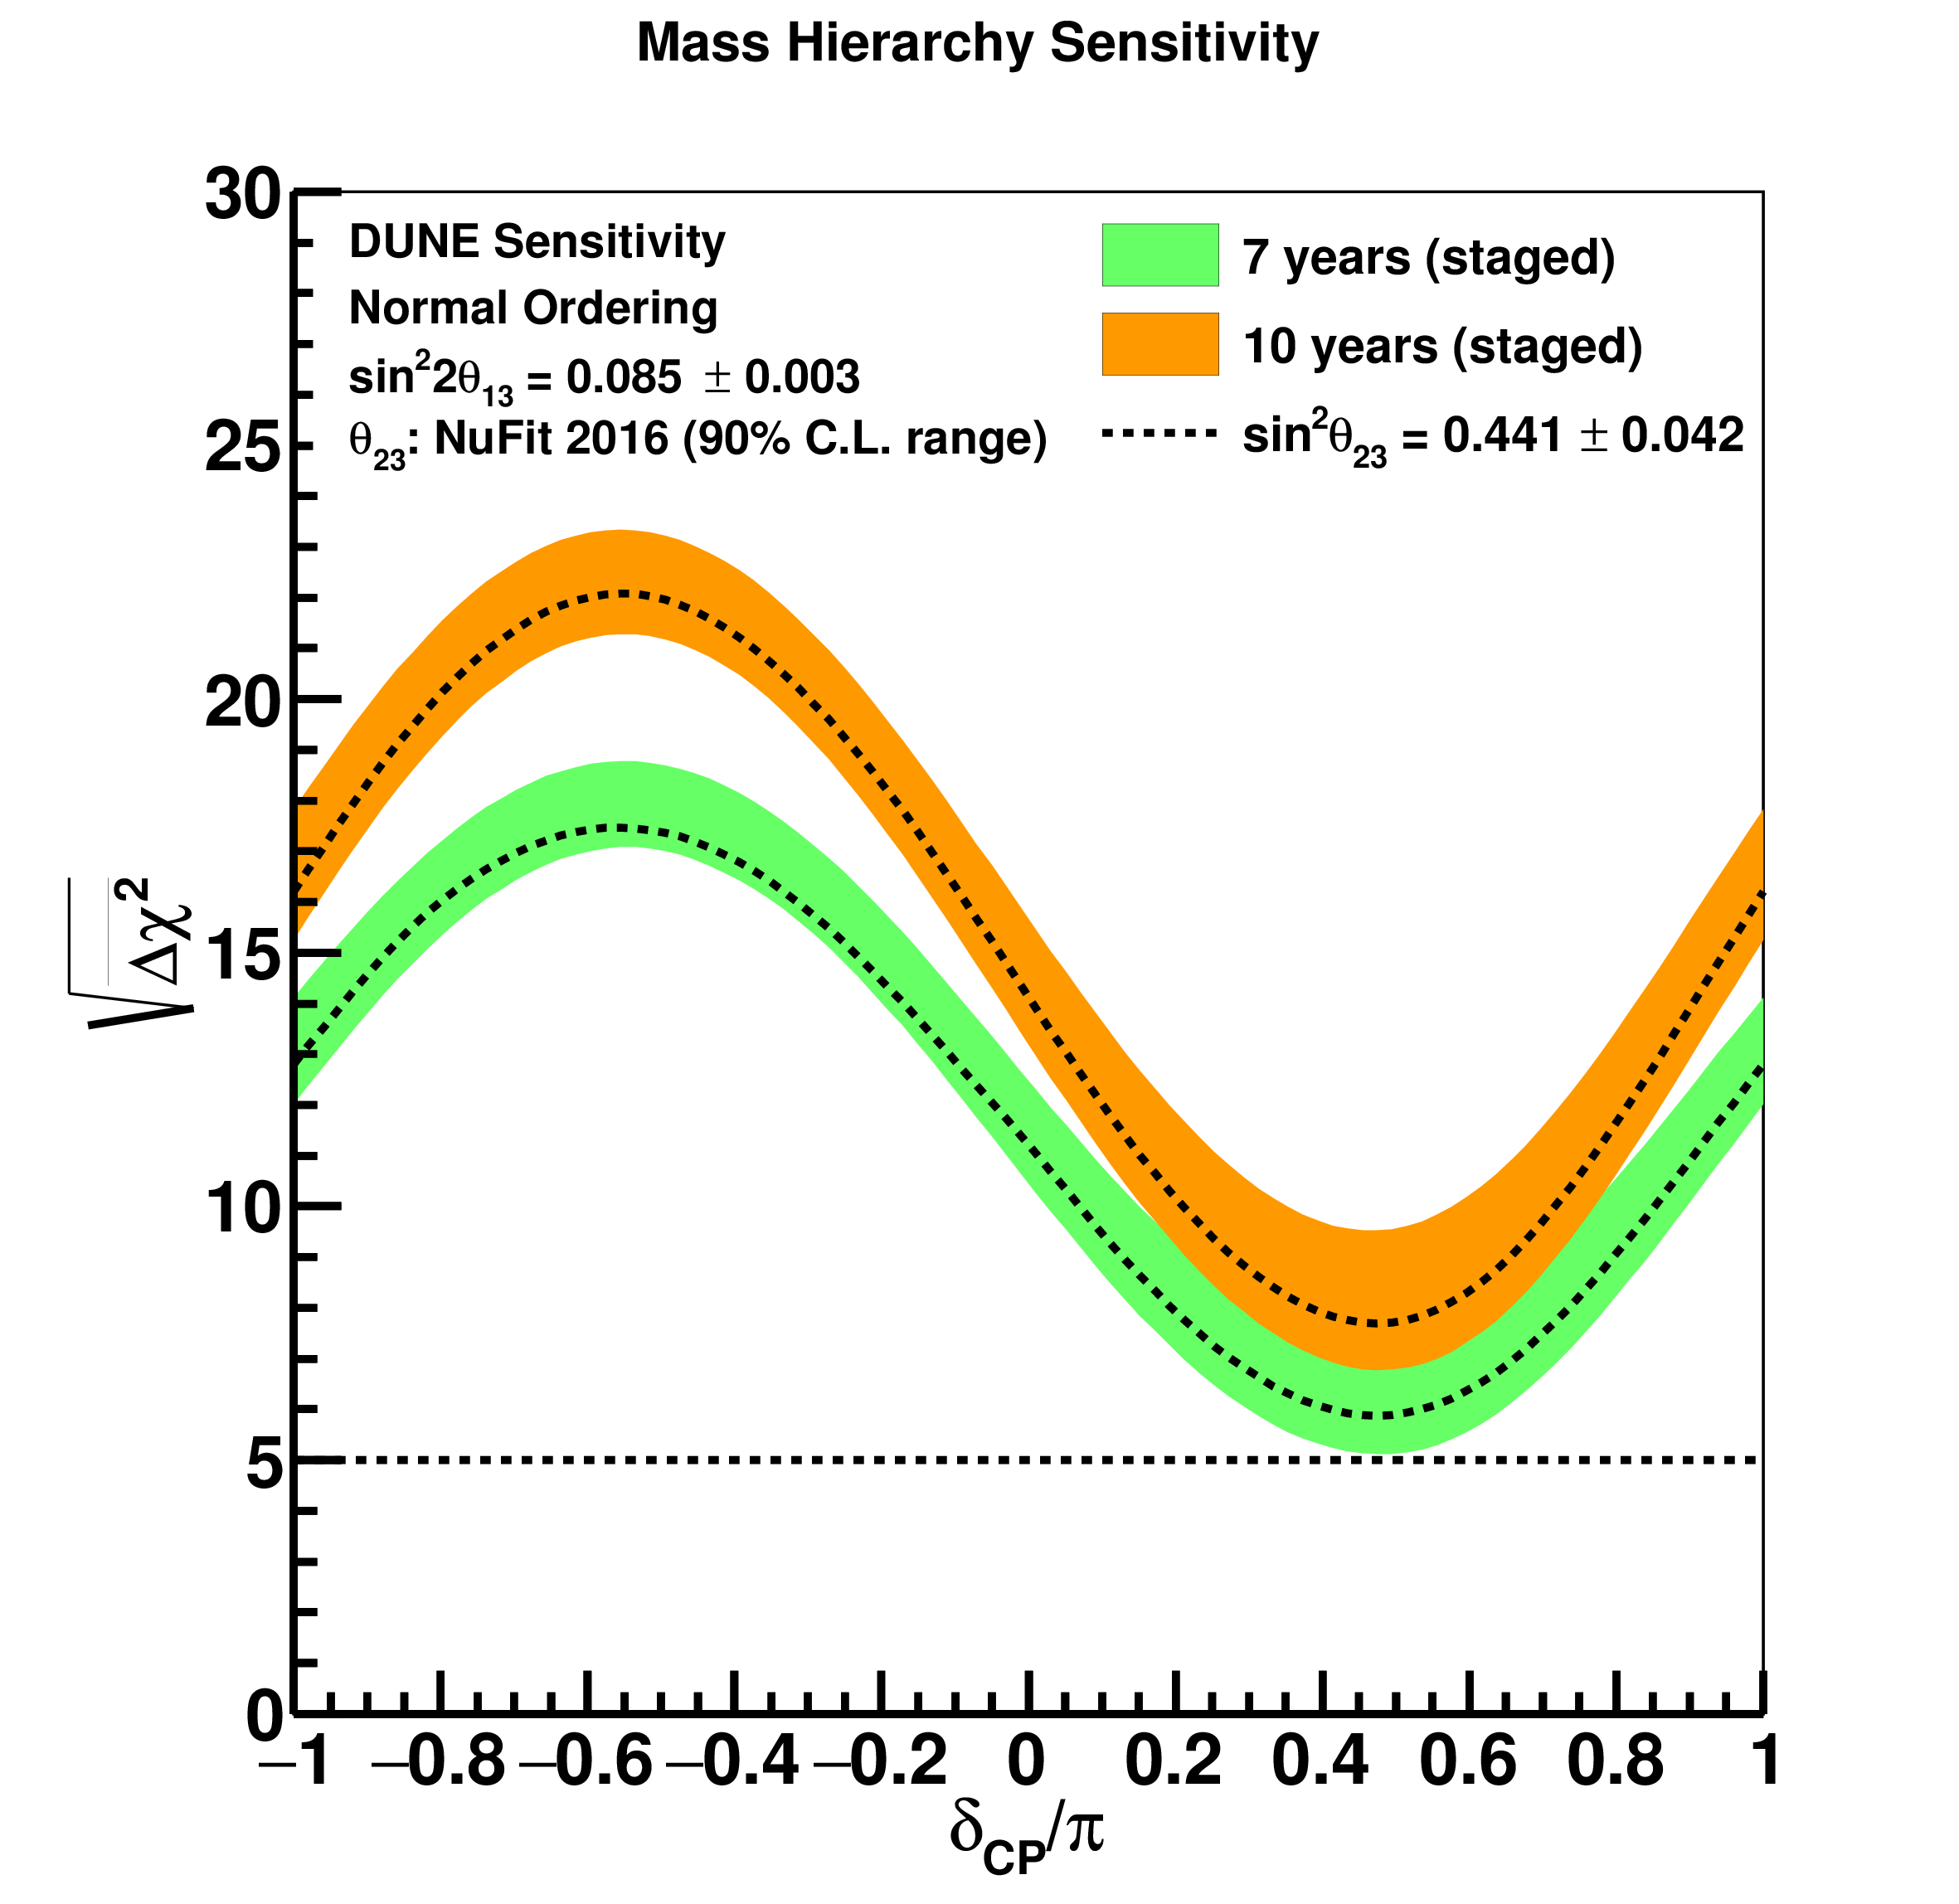
\includegraphics[width=0.47\textwidth]{figs/mh_2017.png}
    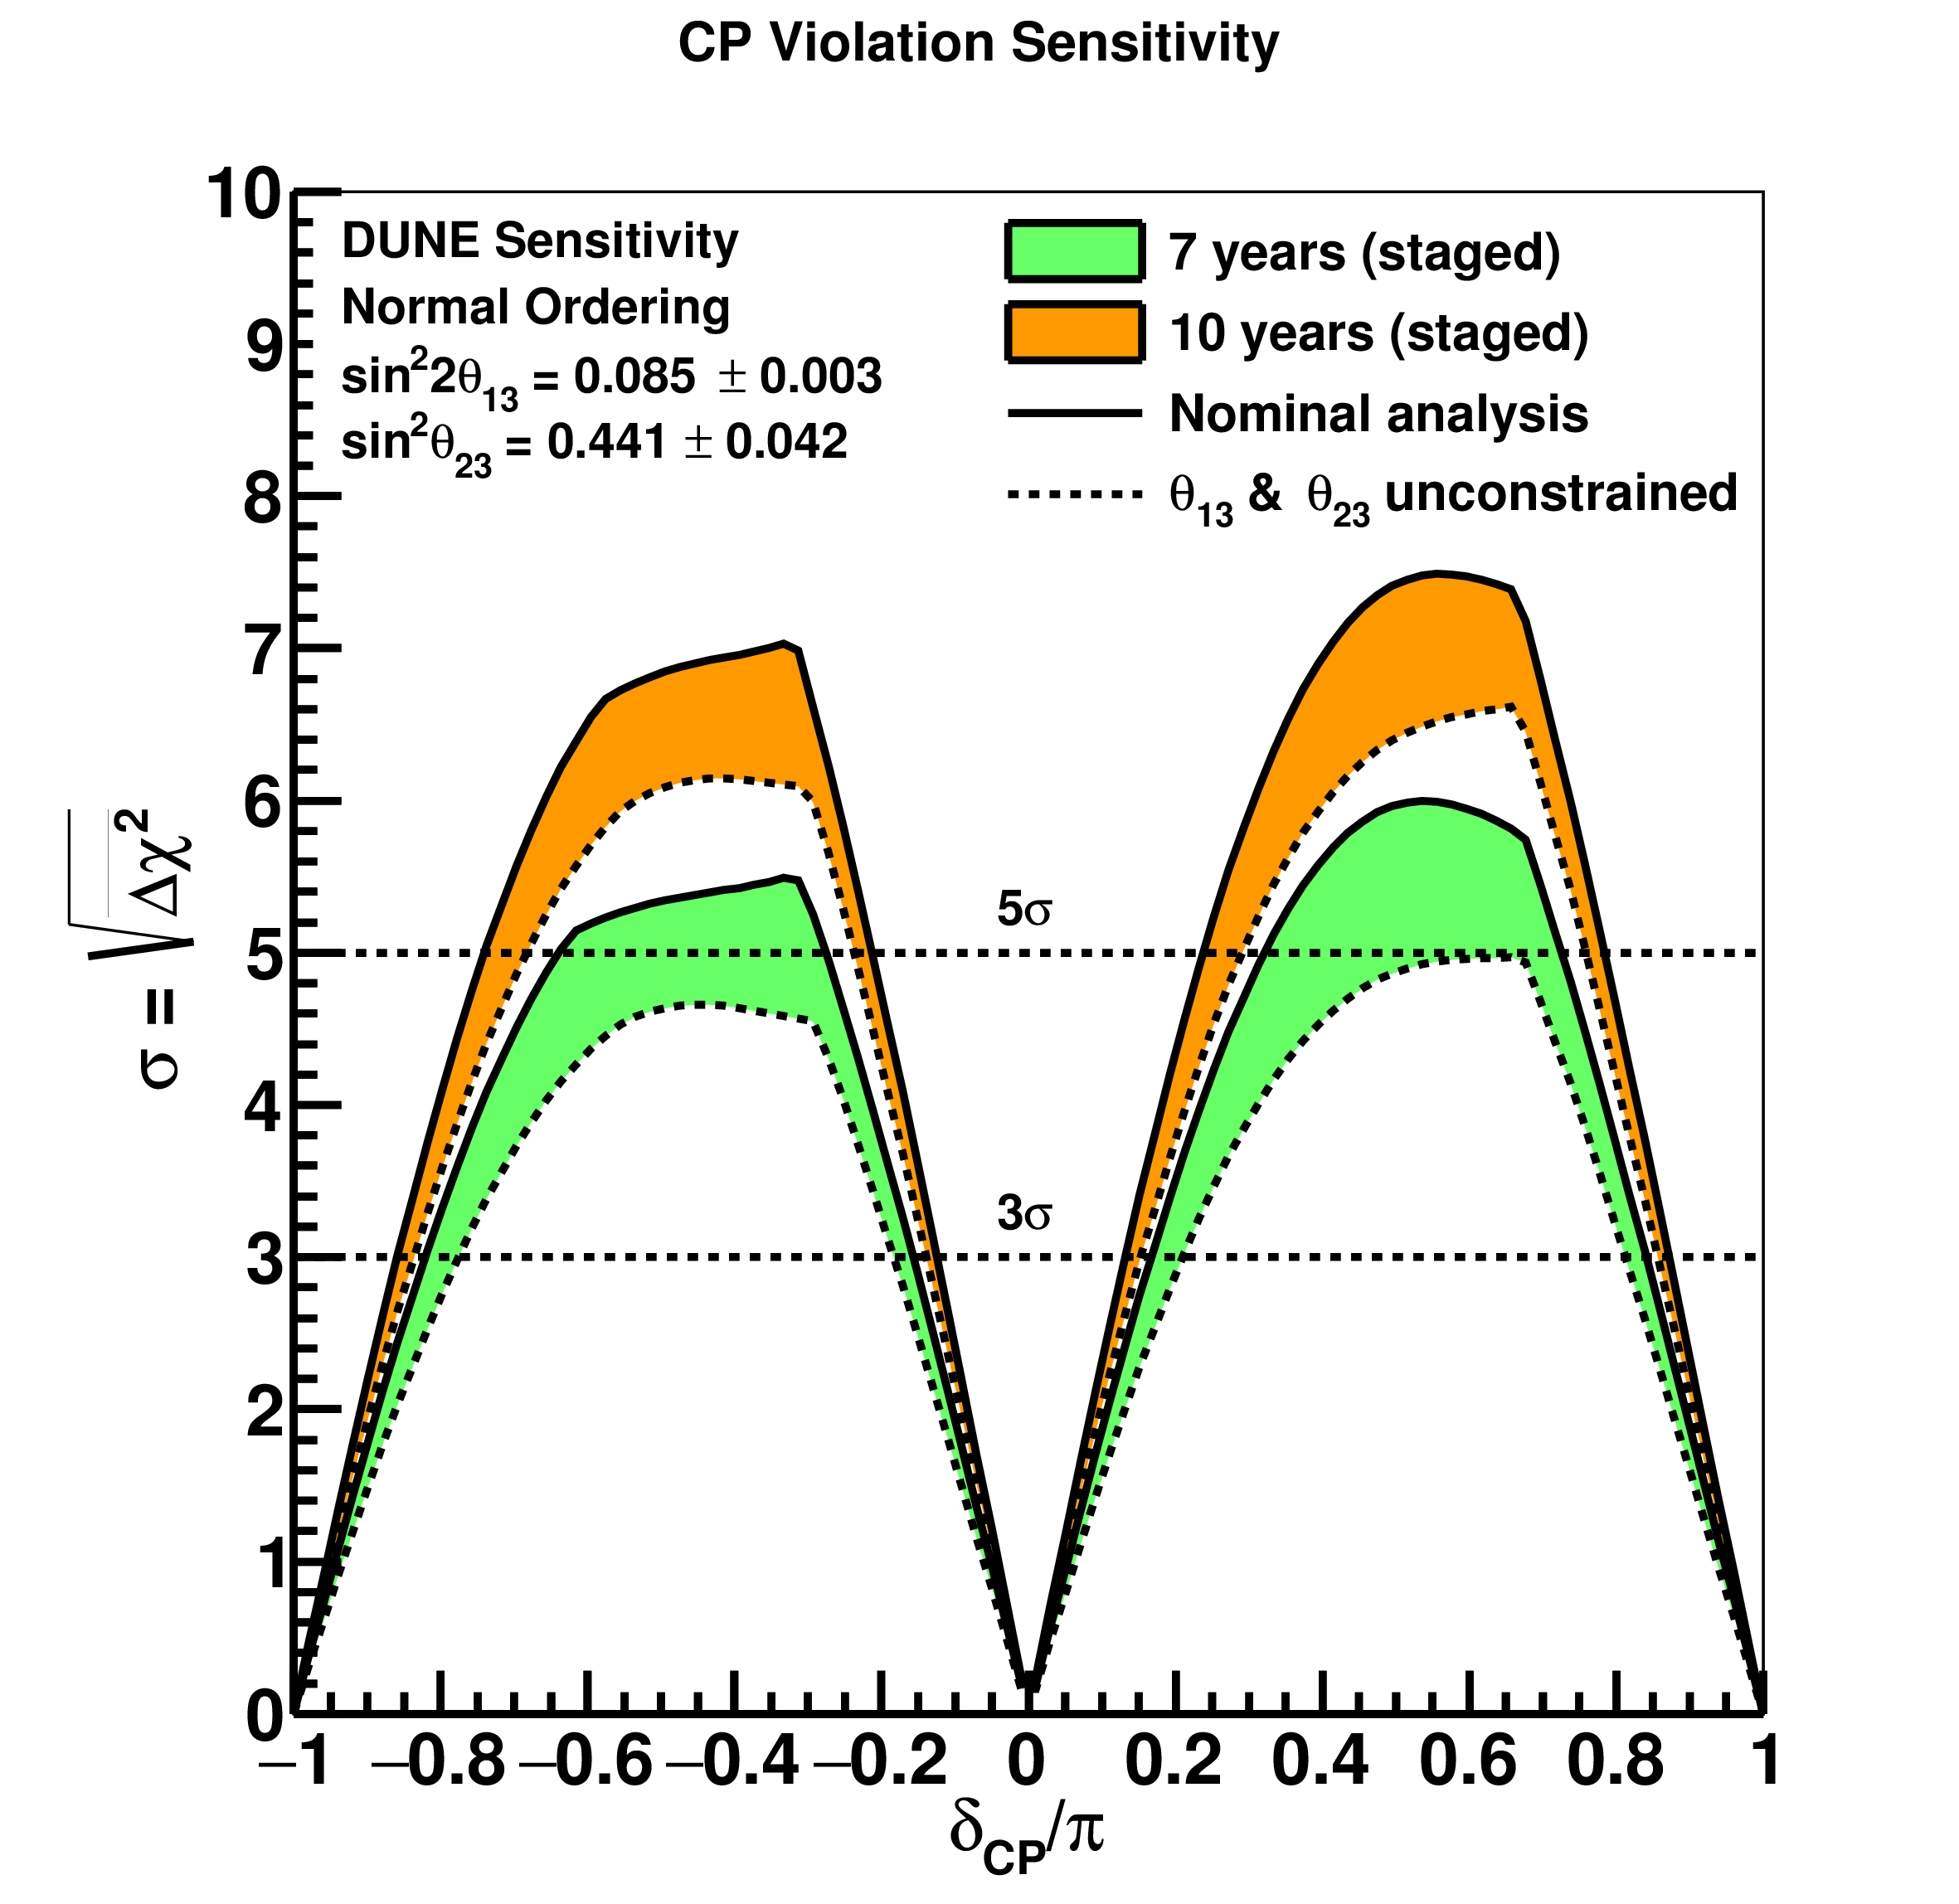
\includegraphics[width=0.47\textwidth]{figs/cpv_2017.png}
    \caption{The plot on the left shows how well DUNE can determine the mass ordering. DUNE will determine the mass ordering independent of the value of all other oscillations parameters with more than 5$\sigma$ after 7 years of running. The right shows the sensitive of how well CP conservation can be excluded as a function of the rue value of $\delta_\text{CP}$ after 7 and 10 years of running.}
    \label{fig:physics}
\end{figure}
 
DUNE will undertake a game-changing programme of neutrino physics, making precision measurements of the parameters that govern $\nu_{\mu} \rightarrow \nu_\text{e}$ and $\overline{\nu}_{\mu} \rightarrow \overline{\nu}_\text{e}$ oscillations. The scientific case for LBNF/DUNE has been presented in detail in volume 2 of the DUNE conceptual design report\cite{2015arXiv151206148D} and only the highest-level scientific goals are repeated here:
\begin{itemize}
\item 
Discovery and measurements of neutrino CP violation. DUNE has $>$3$\sigma$ discovery coverage for 75\% of $\delta_\text{CP}$ values. In favourable regions of parameter space 3$\sigma$ (5$\sigma$) sensitivity can be reached with 3$-$4 (6$-$7) years of operation. Ultimately, $\delta_\text{CP}$ can be measured with a precision of between 7$-$10$^\circ$ (depending on the angle itself), starting to approach the current level for the CP violating angle in the quark sector.   
\item  
Precision neutrino physics, including the definitive determination of the mass hierarchy. Because of the very long baseline, DUNE reaches 5$\sigma$ MO sensitivity within 2$-$5 years 
(depending on the values of other parameters).	
\item
Search for new physics beyond the current understanding of neutrino oscillations. The long-baseline and wide-band neutrino beam will enable DUNE to test the current three-flavour paradigm of neutrino oscillations, providing sensitivity to non-standard neutrino interactions and sterile neutrinos. 
\item 
Observation of the electron neutrino burst from a galactic core-collapse supernova. Unlike in water \v{C}erenkov or liquid scintillator detectors, the main sensitivity in a liquid argon detector is to $\nu_\text{e}$ (rather than $\overline{\nu}_\text{e}$), providing a real-time probe of electron neutrino burst from the initial stage of the neutron star formation phase ($\text{p} + \text{e}^- \rightarrow \text{n} + \nu_\text{e}$). 
\item 
Search for proton decay. Nucleon decay is expected in most models of new physics but has yet to be observed. A large LAr TPC provides an almost background free search for many proton decay modes, including decay modes with kaons.
\end{itemize} 

